% !TEX TS-program = pdflatex
% !TEX encoding = UTF-8 Unicode

\documentclass[12pt]{article} % use larger type; default would be 10pt

\usepackage[margin=1in]{geometry} % fix margins
\usepackage[utf8]{inputenc} % set input encoding (not needed with XeLaTeX)
\usepackage{enumerate}
\usepackage{algorithm}
\usepackage{algorithmic}
\renewcommand{\algorithmicrequire}{\textbf{Input:}}
\renewcommand{\algorithmicensure}{\textbf{Output:}}

\usepackage{graphicx} % support the \includegraphics command and options
\usepackage{tabularx} % allow newlines in table cells
\usepackage{multirow}
\usepackage[parfill]{parskip} % Activate to begin paragraphs with an empty line rather than an indent

%%% PACKAGES
\usepackage{booktabs} % for much better looking tables
\usepackage{array} % for better arrays (eg matrices) in maths
\usepackage{paralist} % very flexible & customisable lists (eg. enumerate/itemize, etc.)
\usepackage{verbatim} % adds environment for commenting out blocks of text & for better verbatim
\usepackage{subfig} % make it possible to include more than one captioned figure/table in a single float
\usepackage{listings}
\usepackage[hyphens]{url}
\usepackage{hyperref}
\usepackage{amsmath}

%%% HEADERS & FOOTERS
\usepackage{fancyhdr} % This should be set AFTER setting up the page geometry
\pagestyle{fancy} % options: empty , plain , fancy
\renewcommand{\headrulewidth}{0pt} % customise the layout...
\lhead{}\chead{}\rhead{}
\lfoot{}\cfoot{\thepage}\rfoot{}

%%% SECTION TITLE APPEARANCE
%\usepackage{sectsty}
%\allsectionsfont{\sffamily\mdseries\upshape} % (See the fntguide.pdf for font help)
% (This matches ConTeXt defaults)

%%% ToC (table of contents) APPEARANCE
\usepackage[nottoc,notlof,notlot]{tocbibind} % Put the bibliography in the ToC
\usepackage[titles,subfigure]{tocloft} % Alter the style of the Table of Contents
\usepackage[titletoc]{appendix} % Put the word "Appendix" in the ToC
\renewcommand{\cftsecfont}{\rmfamily\mdseries\upshape}
\renewcommand{\cftsecpagefont}{\rmfamily\mdseries\upshape} % No bold!

%%% END Article customizations

%%% The "real" document content comes below...

\title{CREATIVE TITLE}
\author{Sean Robbins, Jacob Combs, Matthew Hardwick}
\date{\today}

\begin{document}
\maketitle
\tableofcontents

\section{Problem Statement}
\label{sec:statement}

In graph theory, a \emph{walk} is a sequence of edges connected by vertices. A \emph{self-avoiding walk} is one that can be traced from start to finish without tracing over the same vertex more than once. Put another way, the a walk $w$ is self-avoiding if $w$ does not have any self loops.

A finite automaton can be used to process the set of edges $3\times n$ square lattice. We develop a set of symbols that can be used to encode any such lattice; this symbol set constitutes the input alphabet of the finite automaton that recognizes lattices that contain a self-avoiding walk.

This finite automata accepts $3\times n$ square lattices that meet the following criteria:
\begin{enumerate}
\item The edges of the lattice represent a self-avoiding walk.
\begin{enumerate}
\item Walks in the lattice do not ``jump''; that is, there are exactly two ends, or vertices of degree 1.
\item Walks in the lattice do not ``branch''; that is, no vertex has degree greater than 2.
\item There are no closed loops in the lattice.
\end{enumerate}
\item A walk begins at the ``origin'' (the leftmost, bottom point) of the lattice. This condition not only simplifies the design of the automaton, but also ensures that if the automaton is used to count self-avoiding walks, double-counting the horizontal translations or vertical reflections of the same walk is avoided.
\end{enumerate}


\section{Solution Overview}
Ultimately, we will design a deterministic finite automaton (DFA) $M = \langle Q, \Sigma, \delta, q_0, F \rangle$, where $Q$ is the state set, $\Sigma$ is the input alphabet, $\delta : Q\times\Sigma \rightarrow Q$ is the transition function, $q_0$ is the initial state, and $F\subseteq Q$ is the set of final states.

First, we define the alphabet $\Sigma$. A finite lattice is represented as a sequence of 5-bit binary strings as described in Figure~\ref{fig:encoding-symbol}. We encode the lattice left-to-right. Note that this means for the first (leftmost) symbol $a=a_0a_1a_2a_3a_4$, it must be the case that $a_0 = a_2 = a_4 = 0$, because edges that correspond to these three symbols do not appear on the lattice.

\begin{figure}
\begin{center}
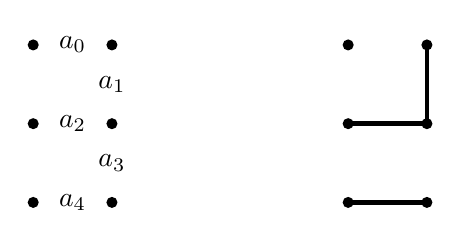
\begin{tikzpicture}
\foreach \x in {0,1}
\foreach \y in {0,1,2}
{
\fill (\x,\y) circle (2pt);
}
\node at (0.5,2) {$a_0$};
\node at (1,1.5) {$a_1$};
\node at (0.5,1) {$a_2$};
\node at (1,0.5) {$a_3$};
\node at (0.5,0) {$a_4$};

\foreach \x in {4,5}
\foreach \y in {0,1,2}
{
\fill (\x,\y) circle (2pt);
}
\draw [ultra thick] (5,2) -- (5,1) -- (4,1);
\draw [ultra thick] (4,0) -- (5,0);
\end{tikzpicture}
\end{center}
\caption{\emph{Left:} Positions of each of 5 bits in the binary string $a = a_0a_1a_2a_3a_4$, a symbol in the alphabet; $a_i = 1$ if there is an edge in position $a_i$, and 0 otherwise. \emph{Right:} Example input symbol $a=01101$ as it appears on the lattice.}
\label{fig:encoding-symbol}
\end{figure}

The finite automaton reads input symbols over the alphabet described above, and determines if they represent a valid self-avoiding walk as defined in Section~\ref{sec:statement}. A state in this automaton is represented by a 4-tuple $q = \langle t, m, b, c\rangle$:
\begin{itemize}
\item Elements $t$, $m$, and $b$ represent the degrees of the top, middle, and bottom (respectively) of the rightmost vertices of the input so far. (Notice that these values depend only on the most recent input symbol.) Because self-avoiding walks do not have branches, we are only interested in states for which $t, m, b \in \{0, 1, 2\}$. Provided the input is a valid walk, the number of ones among $t$, $m$, and $b$ represents the number of vertices that the next input symbol may connect to. We divide states by this characteristic:
\begin{itemize}
\item If a state has a single 1-degree vertex, then we refer to it as \emph{single-ended}.
\item If a state has exactly two 1-degree vertices, then we refer to it as \emph{double-ended}. Notice that if we are in a double-ended state, we must have already seen both ends of the valid walk (because one end is at the origin and to induce a second would otherwise require a branch, which is not allowed).
\item If a state has three 1-degree vertices, then we refer to it as \emph{triple-ended}. For the purpose of identifying closed loops, we require an additional bit of state in the case of triple-ended states because two possible pairs of states may have already been connected; see the description of the $c$ element.
\item If a state has no 1-degree vertices, then we have finished processing the walk and any further input should be trivial in order for the lattice to be valid.
\end{itemize}
\item Element $c$ represents closure information. If the state is single- or double-ended, then $c$ is not needed (so $c=0$ in those cases); if the state is triple-ended, $c$ will be either 1 or 2 depending on which pair of vertices is connected:
\begin{itemize}
\item If the top and middle vertices are connected, then $c=2$.
\item If the middle and bottom vertices are connected, then $c=1$.
\end{itemize}
\end{itemize}

In addition to the states that can be described in the manner outlined above, we will use three auxilliary states: \emph{`start'}, \emph{`done'}, and \emph{`dead'}. We present the complete list of required states in Table~\ref{tab:states}.

\begin{table}
\begin{center}
\begin{tabular}{cccc}
\hline
Single-ended & Double-ended & Triple-ended & Auxilliary \\
\hline
1000 & 1010 & 1111 & \emph{start} \\
1200 & 1210 & 1112 & \emph{done} \\
1220 & 1100 &  & \emph{dead} \\
0100 & 1120 &  &  \\
2100 & 0110 &  &  \\
0120 & 2110 &  &  \\
0010 &  &  &  \\
0210 &  &  &  \\
2210 &  &  &  \\
\hline
\end{tabular}
\end{center}
\caption{All states of interest, categorized by how many 1-degree vertices there are in the set of rightmost vertices. Final states include all the single-ended states, as well as the \emph{`start'} (accept walks of length 0), and \emph{`done'} states.}
\label{tab:states}
\end{table}


\section{Implementation Details}
\label{sec:implementation}

\subsection{Transition function}

In Listing~\ref{lst:delta}, we present the python module that contains documented code for the transition function outlined in Section~\ref{sec:overview-delta}. As the module documentation explains, this code is intended for use with David Eppstein's Python Algorithms and Data Structures (PADS) library~\cite{eppstein:automata:www:2013}, which we used to test it.

This code is also available with additional test code and documentation as a public git repository~\cite{combs:walksoft:www:2013}.

\lstinputlisting[caption=Implementation of transition function $\delta$ in Python.,label=lst:delta]{../delta.py}

\subsection{Visualization}

A tool to help visualize the use of the finite automaton presented in this paper is freely available online~\cite{hardwick:walkvisual:www:2013}. Put simply, it is nothing short of revolutionary.


\section{Sample Input and Output}
When creating test cases to check the validity of the delta function outlined in Section~\ref{sec:overview-delta}. We broke down our test cases to exploit the catagorys of failures on our latice. Our first constraint of the walk having to begin at (0,0) is tested by the the value of the start state, if the walk could pass this it woudd move out to check for jumps, branches and closure properties. A jump on the latice can happen in one of two ways; horizontal or vertical. A branch has many sub-catagories depending on what is a valid input from the next, the idea is that whatever node the state is currently in can only transfer to one or the other but not both. Closure properties test for self avoding walks, so we created test cases that would demonstrate the delta function knew how to proceed. Out of 60 ran cases below are 4 and how they were logically ran through the delta funtion. 

Figure~\ref{fig:test-branch} demonstrates how the branch condition functions in rejecting an unvalid state. After the start state is processed, for this to be a valid walk it must proceed either from the top or bottom, not both. This is because of the condition that the walk must begin at point (0,0). Once the next input is read into the algorithm this would traverse to the dead state. This is because The branch function detected that this input it received has diverged away from a single path. Once the walk is in the dead state the rest immeditly becomes invalid.
\begin{figure}[h!]
\begin{center}
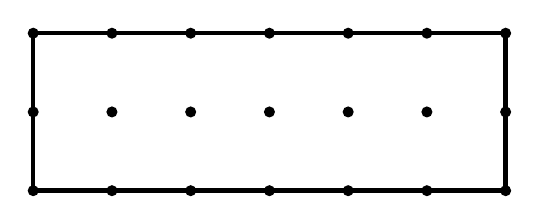
\begin{tikzpicture}
\foreach \x in {0,...,6}
\foreach \y in {0,1,2}
{
\fill (\x,\y) circle (2pt);
}

\draw [ultra thick] (0,0) -- (6,0) -- (6,2) -- (0,2) -- (0,0);

\end{tikzpicture}
\end{center}
\caption{Test case to illustrate branch recognition.}
\label{fig:test-branch}
\end{figure}

Figure~\ref{fig:mult-branch} further shows how the branch condition can detech a unvalid walk. When you receive the input state the only next valid state would be a single node along the bottom. We recvive that making the next valid walk a single node along the top. After the next one however it can easily perceivea branch because it has traversed from the bottom and the middle and not just the top as would have been allowed. This example demonstrates how going from a single node to an illegal triple node is detected.
\begin{figure}[h!]
\begin{center}
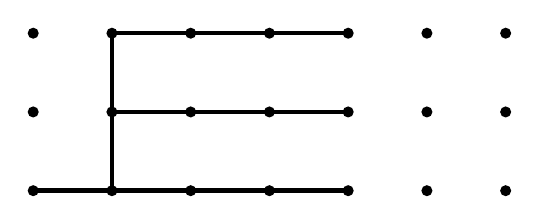
\begin{tikzpicture}
\foreach \x in {0,...,6}
\foreach \y in {0,1,2}
{
\fill (\x,\y) circle (2pt);
}

\draw [ultra thick] (0,0) -- (1,0) -- (2,0) -- (3,0) -- (4,0);
\draw [ultra thick] (1,0) -- (1,1) -- (1,2);
\draw [ultra thick] (1,1) -- (2,1) -- (3,1) -- (4,1);
\draw [ultra thick] (1,2) -- (2,2) -- (3,2) -- (4,2);

\end{tikzpicture}
\end{center}
\caption{Test case to recognize multiple branches}
\label{fig:mult-branch} 
\end{figure}

Figure~\ref{fig:double-ended} is to show how once you have traveled to a double-ended state that you must continue to be in any of these double states for the walk to be valid. When the first input is received after the start state is gets a middle bottom path, at this point for example if the algorithm received an input with C=1 (middle and bottom are connected) it would accept. The walk contiues along the double-ended state and eventualy receives the proper closure andis then accepted.
\begin{figure}[h!]
\begin{center}
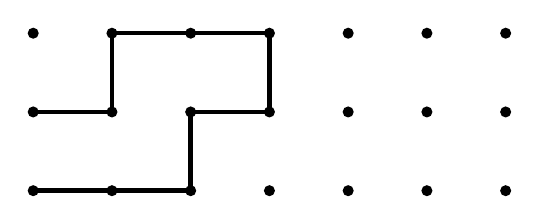
\begin{tikzpicture}
\foreach \x in {0,...,6}
\foreach \y in {0,1,2}
{
\fill (\x,\y) circle (2pt);
}

\draw [ultra thick] (0,0) -- (1,0) -- (2,0) -- (2,1) -- (3,1) -- (3,2) -- (2,2) -- (1,2) -- (1,1) -- (0,1);

\end{tikzpicture}
\end{center}
\caption{Double-ended valid walk}
\label{fig:double-ended}
\end{figure}

Figure~\ref{fig:triple-ended} shows a triple-ended state, a valid input from triple-ended state must connect all the nodes to proceed.After the start stateis read, the first input is another triple-ended state and closes two of the paths. This is a valid and the last input we receive so this is a self-avoiding walk.
\begin{figure}[h!]
\begin{center}
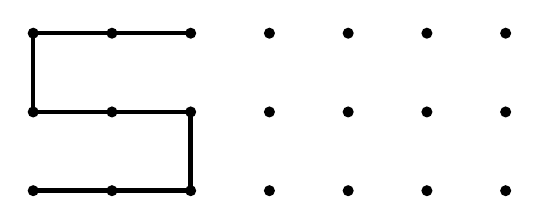
\begin{tikzpicture}
\foreach \x in {0,...,6}
\foreach \y in {0,1,2}
{
\fill (\x,\y) circle (2pt);
}

\draw [ultra thick] (0,0) -- (1,0) -- (2,0) -- (2,1) -- (1,1) -- (0,1) -- (0,2) -- (1,2) -- (2,2);

\end{tikzpicture}
\end{center}
\caption{Tripple-ended}
\label{fig:triple-ended}
\end{figure}


\section{Summary and Conclusions}
Designing the encoding and finite automaton to recognize self-avoiding walks was an iterative process. Our concept of state and alphabet underwent numerous revisions as we tested and re-tested each idea. The result is an algorithm, the transition function $\delta$ outlined in Section~\ref{sec:overview-delta}, that we believe is sound and complete. At each step of the algorithm, we reason that each case discussed is accounted for, and that the complete algorithm accounts for all possible inputs. In addition, we tested the automaton on more than 50 inputs. While the data provide strong evidence that our algorithm is good, this research would be more complete with a formal proof of the algorithm's correctness.

The DFA produced by this algorithm consists of 20 states, and 136 transitions to non-dead states. Using the tools available in PADS~\cite{eppstein:automata:www:2013}, we found that the minimized DFA consists of only 17 states and 126 transitions to non-dead transitions. In fact, evaluation of the minimal DFA reveals that we could simplify our concept of state (presented in Section~\ref{sec:overview-state}) slightly by removing some ``double-ended'' states that were apparently redundant. It is encouraging that we were able to develop a DFA that is so close to minimal without using minimization tools. Furthermore, provided that the algorithm is correct, this slight revision to our concept of state would result in an ``optimal'' algorithm for the transition function in the sense that it would produce a minimal DFA. 

It would be straightforward to use this DFA constrction to count the number of self-avoiding walks in a $3\times n$ square lattice. Counting the number of walks of a given length $k$ is less straightforward, because each input symbol may add a variable number of segments to a valid walk. However, considering the ``weight'' of each input symbol in terms of the length it adds to the self-avoiding walk is likely a good place to start.


%\bibliographystyle{acm}
%\bibliography{report}

\end{document}
